\part{Énonciation et motifs}

\chapter{L'Énonciation}

\section{Propos liminaires}

Après avoir procédé à différentes analyses assez traditionnelles (avec les approches complémentaires supervisées et non-supervisées) en humanités numériques pour défricher nos textes pamphlétaires et faire émerger ou plus simplement constater quantitativement certains rapprochement de nos pamphlets avec différents genres, nous souhaitons dans cette partie interroger directement des aspects distinctifs du genre pamphlétaire. Cela va se faire avec la présentation de deux analyses, l'une portant sur l'énonciation pamphlétaire, l'autre sur la recherche de motifs. L'énonciation pamphlétaire, déjà occultée par Marc Angenot dans son travail que nous citons toujours, \enquote{\textit{La parole pamphlétaire}}, déploie un discours précis sur la relation du locuteur-narrateur de l'allocutaire et de l'adversaire : le \enquote{je}, le \enquote{vous} qui forment un \enquote{nous} face à un \enquote{il}.  Nous analyserons cela en cherchant quantitativement à définir une spécificité du pamphlet dans son emploi des pronoms. La recherche de motifs génériques, inspirée du travail de Thierry Poibeau et al. sur le cliché amoureux \footcites{legallois_reperer_2016}, nous permettra de chercher des structures génériques au seins des phrases.


\section{Définition énonciation}

L'énonciation en stylistique et dans les principes de la pragmatique est d'un grand secours pour définir certaines spécificités du pamphlet comme genre littéraire. L'énoncé littéraire est pris comme moyen et résultat d'un acte de parole qui suppose plusieurs instances. Le pamphlet genre complexe partage plusieurs caractéristiques de l'énonciation avec d'autres genres comme le discours délibératif, l'essai polémique et l'article journalistique. De l'énonciation de l'essai polémique, le pamphlet est associé a l'ensemble du genre agonique (ou littérature de combat). Le pamphlet est surtout un discours agressif et violent, énonçant régulièrement l'image d'un contre-discours à réfuter et disqualifier. Cette disqualification propre à la polémique dans le cadre du pamphlet s'étend à la disqualification totale d'un adversaire car existe alors un scandale de la Vérité à révéler. Le pamphlet porte aussi un discours persuasif, l'énonciateur veut persuader le destinataire d'une vérité qu'il juge travesti, en ce sens il conserve certaine caractéristique du genre délibératif. Le pamphlétaire destine son discours à deux auditoires distincts, l'un étant un destinataire universel que l'on persuade et l'autre étant un adversaire que l'on disqualifie. Cette double destination du pamphlet complexifie le schéma de l'énonciation qui distingue le genre de ses proches parents: la polémique et la satire. Autrement dit le discours instaure une opposition entre deux adversaires le pamphlétaire et sa cible dont celle-ci est portée à l'arbitrage d'un second destinataire. Sur le plan pragmatique, le discours vise à gagner ce tiers à la cause de l'énonciateur, contre son adversaire, et il se définit ainsi, pour reprendre la terminologie jakobsonienne, par une dominante conative \footcites{jakobson_essais_1963} - je me réfère en particulier au chapitre.11, « Linguistique et poétique » -, que nous allons développer après avoir défini le rôle du locuteur. 

Pour mieux cerner les enjeux de l'énonciation propre au pamphlet nous allons définir les différentes instances entre le locuteur et les deux allocutaires repérés.

\subsection{Définir l'énonciation pamphlétaire : Le locuteur}

L'énonciation dans le genre pamphlétaire semble jouir d'un statut complexe. Le pamphlet a ceci de commun avec l'ensemble des énoncés littéraires, du fait qu'il joue avec la langue et que l'évidence de l'énonciation que l'allocutaire reçoit doit être considéré sérieusement.  L'énonciation est un acte de parole dont l'énoncé en est le moyen et le résultat. Cette énonciation dans le pamphlet met en avant un locuteur toujours explicitement présent. En ce sens, on peut la rapprocher du genre des mémoires où la distance entre auteur, narrateur et personnage est volontiers effacée. Le pamphlétaire parle en son nom propre avec sa propre voix. Mais il n'est pas possible de croire à une véritable fusion des trois instances (auteur, narrateur, personnage) car il existe un dédoublement du \enquote{je}. Les pamphlets demeurent des textes extrêmement construits et pensés. L'instance autoriale du \enquote{je} écrit pour un \enquote{je} narrateur situé dans un autre temps et dans espace, l'auteur remanie et retravaille ce qu'il narre. Si la distance entre ces instances parait minime, c'est que l'énoncé pamphlétaire est issu d'un contrat d'authenticité similaire au pacte autobiographique \footcites{lejeune_pacte_1975}. Bernanos en incipit de \textit{La Grande Peur des Bienpensants} écrit par exemple : \\
	
	\enquote{J'écris ce livre pour moi, et pour vous — pour vous qui me lisez, oui : non pas un autre, vous, vous-même. J'ai juré de vous émouvoir — d'amitié ou de colère, qu'importe ? Je vous donne un livre vivant.}\\

Bernanos auteur s'affirme en tant qu'énonciateur explicite avec l'usage du \enquote{je}. Les trois verbes conjugué à la première personne du singulier sont \enquote{écrire}, \enquote{jurer} et \enquote{donner}, ils marquent la performativité du propos, cette exemple agit comme un contrat.

	\enquote{1) POURQUOI JE PUBLIE CE LIVRE. — Je n'avais jamais soupçonné qu'aucun travail de lettres me donnerait la répugnance que je dois surmonter pour rassembler les feuillets de ce livre[...] Chacun des articles que réunit ce volume fut l'expression spontanée et minutieusement exacte des mouvements de mon âme. J'ai vécu, et je ne voudrais point avoir vécu autrement.}\footcites{barres_scenes_1902}\\


Le genre du pamphlet partage un même brouillage de rapport entre l'auteur et le narrateur que celui du genre autobiographique. Le locuteur veut paraître d'un bloc auteur et narrateur, c'est un enjeu d'authenticité et de sincérité de ce qui est dit.\\

	\enquote{J'écris ce que je pense, mais je ne l'écris pas pour mon plaisir. Voilà même pourquoi je me hâte de l'écrire, je sais parfaitement que le temps m'est mesuré.}\footcites{bernanos_francais_1961}\\
	
En cela, le pamphlet porte une ambiguïté similaire au genre épistolaire où la sincérité de ce qui est narré est garanti par un pacte de même facture que celui propre au genre autobiographique. Il faut aussi noter que le \enquote{je} qui s'exprime n'est donc pas fictionnel comme au théâtre ou comme en poésie avec le \enquote{je} lyrique. \\

	\enquote{Croyez-vous donc que j'eusse voulu être entendu de n'importe qui? J'écrivais pour mettre de l'ordre en moi-même et pour me délivrer, car on ne pense, ce qui s'appelle penser, que la plume à la main. Mais le premier venu allait-il pencher sa tête, par-dessus mon épaule, sur mon papier ?}\footcites{barres_homme_1889}\\
	
Si l'on ne peut sonder les coeurs ni les reins au sujet de la sincérité de ce qu'ont pensé et écris les pamphlétaires, l'on constate néanmoins que tous insistent sur la sincérité de leur propos. S'il y a feinte de leur sincérité cela est volontairement effacé. \\

	\enquote{J'ai eu le dégoût d'entendre un ministre de l'instruction publique amuser la Chambre avec des plaisanteries sur le Moi de M. Barrès.[...] Cette après-midi me montra clairement que pour agir sur des intelligences la sincérité ne suffit pas.} \footcites{barres_homme_1889}\\

Qu'il y eu des spécialistes du pamphlet comme des spécialistes d'autres genres tel que dans le journalisme, cela pourrait faire penser que comme toute professionnalisation en littérature, celle de l'indignation lucrative peut demander de feindre des propos pour vivre. Octave Mirbeau au début de sa carrière écrivait qu'il était un \enquote{\textit{prolétaire des lettres}}.
Et Georges Bernanos d'écrire en préface du \textit{Crépuscule des Vieux} : \\
	
	\enquote{Mais les livres sincères ne sont pas les plus faciles à défendre, et vous savez que j'ai écrit celui-ci avec une imprudente bonne foi. [...] Quand on arrache ainsi un livre de soi, ligne après ligne, on peut compter qu'il est sincère [...] L'auteur de mauvaise foi se défend par les textes, qu'il est toujours facile de solliciter. Pour moi je dirai seulement mes intentions.} \footcites{bernanos_crepuscule_1956}

Pour développer sur la sincérité feinte, il est un cas connu de mystification chez les pamphlétaires. C'est celui de Léo Taxil, ayant bâti sa carrière du côté des écrivains radicalement anti-cléricaux, il fit une fausse volte face avec les \textit{confessions d'un ex-libre penseur} où il pu raconter sa vie à travers le regard d'un converti pleins de contrition. Après une suite d'essais traitant d'un complot maçonnique fantasmé et ayant acquis à sa cause une partie de l'opinion catholique, il révéla son imposture et repris ses premières positions. Avec ses confessions feintes, nous pouvons remettre en cause le pacte autobiographique, fruit d'une contrefaçon volontaire.

\subsection{Énonciation de l'allocutaire}

Après avoir cerné le statut du locuteur, nous savons qu'avant tout un locuteur est un allocuteur, c'est-à-dire que celui qui écrit, écrit pour quelqu'un. Les principes de la pragmatique vont être appliqués pour analyser les instances réceptrices du pamphlet. Notamment au travers des visées illocutoire de la parole définie par Austin dans \textit{Quand dire, c'est faire}\footcites{austin_quand_1970} et développé par O. Ducrot dans \textit{Le Dire et le Dit, Éd. de Minuit, Paris 1984}.

Mais dans le genre agonistique, l'énonciation s'établit avec une triple relation, en effet il y a deux instances réceptrices distinctes : un discours à dénoncer et un témoin à persuader.
La polémique est justement un contre-discours, en cela elle inverse l'habitude des relations d'intertextualité de la littérature classique, au sens où le pamphlétaire ne cite pas en hommage mais dans le but de réfuter et de rabaisser. Aussi cela amène à penser que le pamphlet n'est pas un texte clos et autonome mais bien à l'inverse en prise dans une toile intertextuelle circonstanciée dans le temps. 

La fonction conative du pamphlet régit l'adresse aux allocutaires liés à la fonction conative de la polémique qui se décompose en fonction adversative associé à l'adversaire – dont le pamphlet se veut être le contre-discours – et en fonction conjonctive associé au destinataire. Ces deux fonctions décrites comme distinctes ne sont pas pour autant dissociables, une même invective aura une visée illocutoire différente en fonction de l'instance réceptrice de l'énoncé : l'adversaire pourra être humilié et le allocutaire susceptible de s'identifier aux positions du locuteur pourra en retirer un plaisir sadique. Cette stratégie d'énonciation suppose qu'il existe un allocutaire pour accepter de jouer le rôle de témoin complice de l'énonciateur qui lui est assigné et d'adhérer au discours de celui-ci au risque de se voir dégrader au premier plan de la réception qui est celui du destinataire-adversaire méprisé.
Reprenons l'extrait de l'incipit de Bernanos de \textit{La Grande Peur des Bienpensants} : \\
	
	\enquote{J'écris ce livre pour moi, et pour vous — pour vous qui me lisez, oui : non pas un autre, vous, vous-même. J'ai juré de vous émouvoir — d'amitié ou de colère, qu'importe ? Je vous donne un livre vivant.}\\

Pour ce qui est de l'identification de l'allocutaire, nous retrouvons le pronom personnel de la deuxième personne du pluriel employé de nombreuses fois à chaque verbe conjugué. Les dédoublements répétitifs du \enquote{vous} participe d'une insistance à désigner expressément l'allocutaire. Sur la diversité de l'allocutaire, bien que Georges Bernanos semble cibler précisement un allocutaire répond à certains critère, l'allocutaire adversatif apparaît sous \enquote{d'amitié ou de colère}, deux postures possibles résultant de la lecture. Nous avons donc dans cette extrait d'incipit l'exemple parfait de cette triple relation du \enquote{je} pamphlétaire parlant pour un \enquote{vous} face à un \enquote{vous} adversatif qui se transformera en \enquote{il}, c'est ce qui conditionne la visée illocutoire entre amitié ou colère de ce qui est écrit.a

\chapter*{Application de la méthode}

\section{Méthodes numériques déployées}

Depuis notre corpus 2 des textes de tout genre de nos auteurs pamphlétaires, nous allons effectuer un comptage des occurrences des pronoms pour constater des variations de l'usage de ceux-ci par genre. Nous regroupons l'ensemble des pronoms personnels, réfléchis et possessifs dans une seule catégorie de nombre que nous pouvons retrouver à la \textit{table \ref{listepronoms}}. Nous souhaitons obtenir des figures boites à moustaches montrant les occurrences par genre de l'occurrence des pronoms.

\begin{table}[ht]
    \centering 
    \begin{tabular}{l c c c c c c c c}
        \toprule
        1st sing & je & j' & me & m' & moi & mon & mes & \\
        \midrule
        2nd sing & tu & t' & te & t' & toi & ton & ta & tes\\
        \midrule
        3rd sing & il & elle & lui & se & soi & son & sa & ses\\
        \midrule
        1st plur & nous & notre & & & nos & & &\\
        \midrule
        2nd plur & vous & votre & & & vos & & &\\
        \midrule
        3nd plur & ils & elles & eux & & & leurs & & \\
        \bottomrule
    \end{tabular}
\caption{Liste des pronoms recensés par personne}
\label{listepronoms}
\end{table} 

\section{Résultats et analyse}

La \textit{figure \ref{sortieboitemoustachepronoms}} montre la proportion d'emploi des pronoms par nombre et par genre. Plus la boite à moustaches dense plus les valeurs des occurrences sont centrés à la moyenne et plus la boite est étirée plus nous pouvons constater une grande diversité de l'occurrence d'un pronom dans un genre donné. Pour la première personne du singulier, nous trouvons sans surprise une plus grande fréquence pour la littérature de l'intime, c'est à dire les mémoires et biographies que pour les autres genres. Le pamphlet lui se situe au même niveau que les genres de l'essai et de l'article. Pour la deuxième personne du singulier, les fréquences sont globalement les mêmes excepté pour le roman qui probablement du fais de la présence de dialogue a une fréquence plus élevée. L'emploi de la troisième personne du singulier est pour le pamphlet assez similaire à la littérature de l'intime et est assez dense. Ce sont les personnes pluriels qui montrent une grande variabilité de fréquence pour les textes pamphlétaires, nous le constatons par l'étalement extrême des boites à moustaches. Nous pouvons voir que la troisième personne pluriel est, en terme de fréquence d'emploi, supérieur à l'ensemble des autres genres. 

\begin{figure}[H]
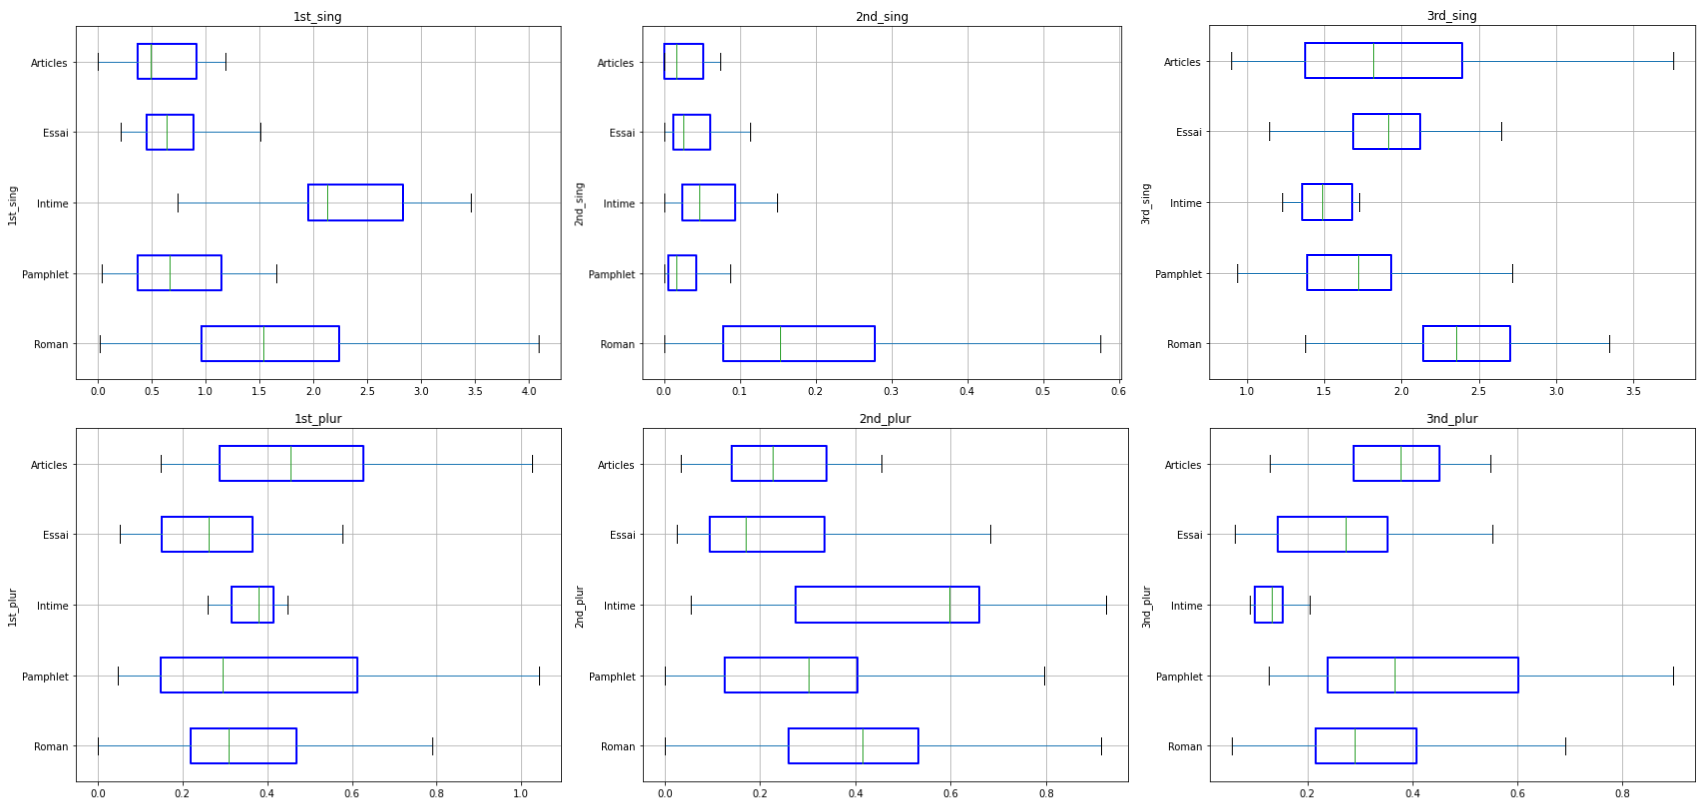
\includegraphics[width=1\textwidth]{img/boxplot_pronoms.png}
\caption{Boite à moustache de la fréquence relative des genres par pronoms}
\label{sortieboitemoustachepronoms}
\end{figure}

\section{Conclusion}

Les résultats ne montrent pas entre le pamphlet et l'essai de différente flagrante sur l'emploi des pronoms. Nous aurions souhaité pouvoir approfondir cette analyse avec la recherche de syntagme plus complexe tel que les suites de \enquote{pronom pronom verbe conjugé} pour avoir un regard plus fin sur la relation des différentes instance de la locution. Avec la librairie Spacy en python, il est possible de rechercher des occurences de \enquote{part-of-speech} ou \enquote{partie de discours} commme avec : \par

    \enquote{[{"TEXT": {"in":["je","tu","il","elle","nous","vous","ils","elles"]}}, {"TEXT": {"in": ["me", "m'","te","t'","le","l'","lui","la","nous","vous","les","s'","leurs"]}}, {"POS":"VERB"}],}

Nous aurions obtenu une matrice combinatoire de tous les emplois des doubles pronoms personnels avant une verbe. Cela aurait pu permettre une analyse factorielle pour discriminer les genres sur l'enjeu de l'énonciation.

\chapter{Recherche de \enquote{motifs} génériques}

\section{Définition des \enquote{motifs}}

Cette seconde partie s'attèle à définir et détecter des motifs distinctifs du genre pamphlétaire. Cela passe par la detection d'occurences lexico-grammaticales caractérisant le style collectif des pamphlétaires. Nous nous appuyons sur le travail de D. Legallois, T. Charnois et T. Poibeau sur l'application de la méthode des motifs du clichés dans les romans sentimentaux\footcites{legallois_reperer_2016}. L'intérêt de cette méthode de detection tient à ce que les formes du cliché sont justement un signe distinctif du roman sentimental\footcites{van_cranenburgh_cliche_nodate}. Pour ce qui est du genre pamphlétaire, nous pensons que le registre polémique et le recours à l'invective puisse être le lieu de formules (motifs) lexicales et grammaticales partagé par une majorité des textes du genre. Nous appliquerons donc une méthode similaire à celle de l'article sur \footcites{legallois_reperer_2016}. Si le cliché est une forme fixe et figée, les auteurs recourt aussi à la detection de forme souple avec des patrons syntaxiques partageant des classes lexicales. \par
Nous appelons \enquote{motifs} des ngrams qui se suivent et se répètent dans un texte ou un corpus de texte. Thierry Poibeau et al.\footcites{legallois_reperer_2016} ont traité cette question des motifs autour du cliché dans les romans sentimentaux. Nous nous inspirons de ce travail pour dans notre cas rechercher des motifs qui soient propres aux textes de pamphlet. Les motifs peuvent être les ngrams de mots mais il est plus intéressant des généraliser l'approche des motifs en modifiant les mots lexicalisés en \textit{part-of-speech}, c'est-à-dire par nature des mots grammaticales. Nous remplaçons dans le corpus de texte les noms, adjectifs, verbes et noms propres en l'indication de leur nature de mots. Cela ajoute une souplesse à la recherche générique de motifs.

\section{Méthode choisie et préparation d'un corpus spécifique}

Pour réaliser cette recherche de motifs nous allons générer nos textes avec la grammaticalisation des noms, adjectifs, verbes et noms propres. Nous effectuons cela avec la librairie Spacy en python. Nous avons tester différents longueur de nombre de mots, les sexto-grammes de mots semblent être le meilleur compromis entre les ressources allouables au calcul et la bonne généralisation de la SVM. Voici un exemple de la sortie des textes avant et après modification : \par

\enquote{Oui, mon Dieu, pour quoi faire, la liberté ? Et pour quoi faire, les pays libres ou réputés tels, la France et ses sœurs d’Europe, pour qui cet idéal de liberté constitue le principal héritage des vieilles chrétientés européennes ?}\textit{La Liberté pour quoi faire ?}, Bernanos\par

\enquote{NOUN , mon PROPN , pour quoi VERB , la NOUN ? Et pour quoi VERB , les NOUN ADJ ou ADJ ADJ , la PROPN et ses NOUN PROPN , pour qui cet ADJ de NOUN VERB le ADJ NOUN des ADJ NOUN ADJ ?}\textit{La Liberté pour quoi faire ?}, Bernanos\par

Nous entraînons avec Superstyl un modèle pour généraliser la classification des textes. Nous extrayons les motifs reconnus comme les plus pertinent pour définir le pamphlet. Nous rechercherons dans les textes la liste des motifs non grammaticalisé en espérant pouvoir analyser une composante stylistique commune.
Pour appliquer cette méthode, nous ne conservons que trois ensemble du corpus 2 défini précédemment, c'est à dire les essais, les romans et les pamphlets de nos auteurs pamphlétaires. Nous délaissons les nouvelles, mémoires et biographies ainsi que les articles car leur distinction avec les pamphlets est plus facilement établi. Nous conservons le roman comme référence très éloignée et le genre de l'essai pour leur grande proximité avec le pamphlet (ce que nous constations précédemment). Pour équilibrer nos classes nous échantillonnons les textes tous les 10000 mots.


\section{Résultats et analyse}

Les résultats de la SVM de la \textit{table \ref{'tab:SVMcorpus2restreint'}} avec les sextogrammes de mots, dont les mots lexicalisés sont grammaticalisés, sont moins bons que ce que nous avons pu obtenir avec les trigrammes de mots simples. Les classes essai et pamphlet sont les moins bien reconnues, néanmoins leurs f1-score restent suffisant pour considérer que le modèle reconnaît les sextogrammes comme cohérent pour généraliser une classification.

\begin{table}[H]
    \centering 
    \begin{tabular}{l c c c c}
        \toprule
             & precision & recall & f1-score & support \\
        \toprule
        \midrule
        roman & 0.87 & 0.92 & 0.90 & 612 \\
        \midrule
        essai & 0.71 & 0.72 & 0.72 & 270\\
        \midrule
        pamphlet & 0.77 & 0.67 & 0.72 & 284\\
        \midrule
        & & & & \\
        \midrule
        accuracy & & & \textbf{0.81} & 1166 \\
        \midrule
        macro-average & 0.79 & 0.77 & 0.78 & 1166\\
        \midrule
        weighted average & 0.81 & 0.81 & 0.81 & 1166\\

        \bottomrule
    \end{tabular}
\caption{Sortie de la SVM sur corpus 2 restreint échantillonné, 6grammes de motifs, LOOCV, class-weight}
\label{'tab:SVMcorpus2restreint'}
\end{table} 
Nous prenons les sextogrammes les plus spécifiques du genre du pamphlet distinct de la classe essai et roman que nous observons sur la figure \ref{'fig:coefs_pamphlet_corpus2restreint'} des coefficients du modèle SVM. 

\begin{figure}[H]
\centering %
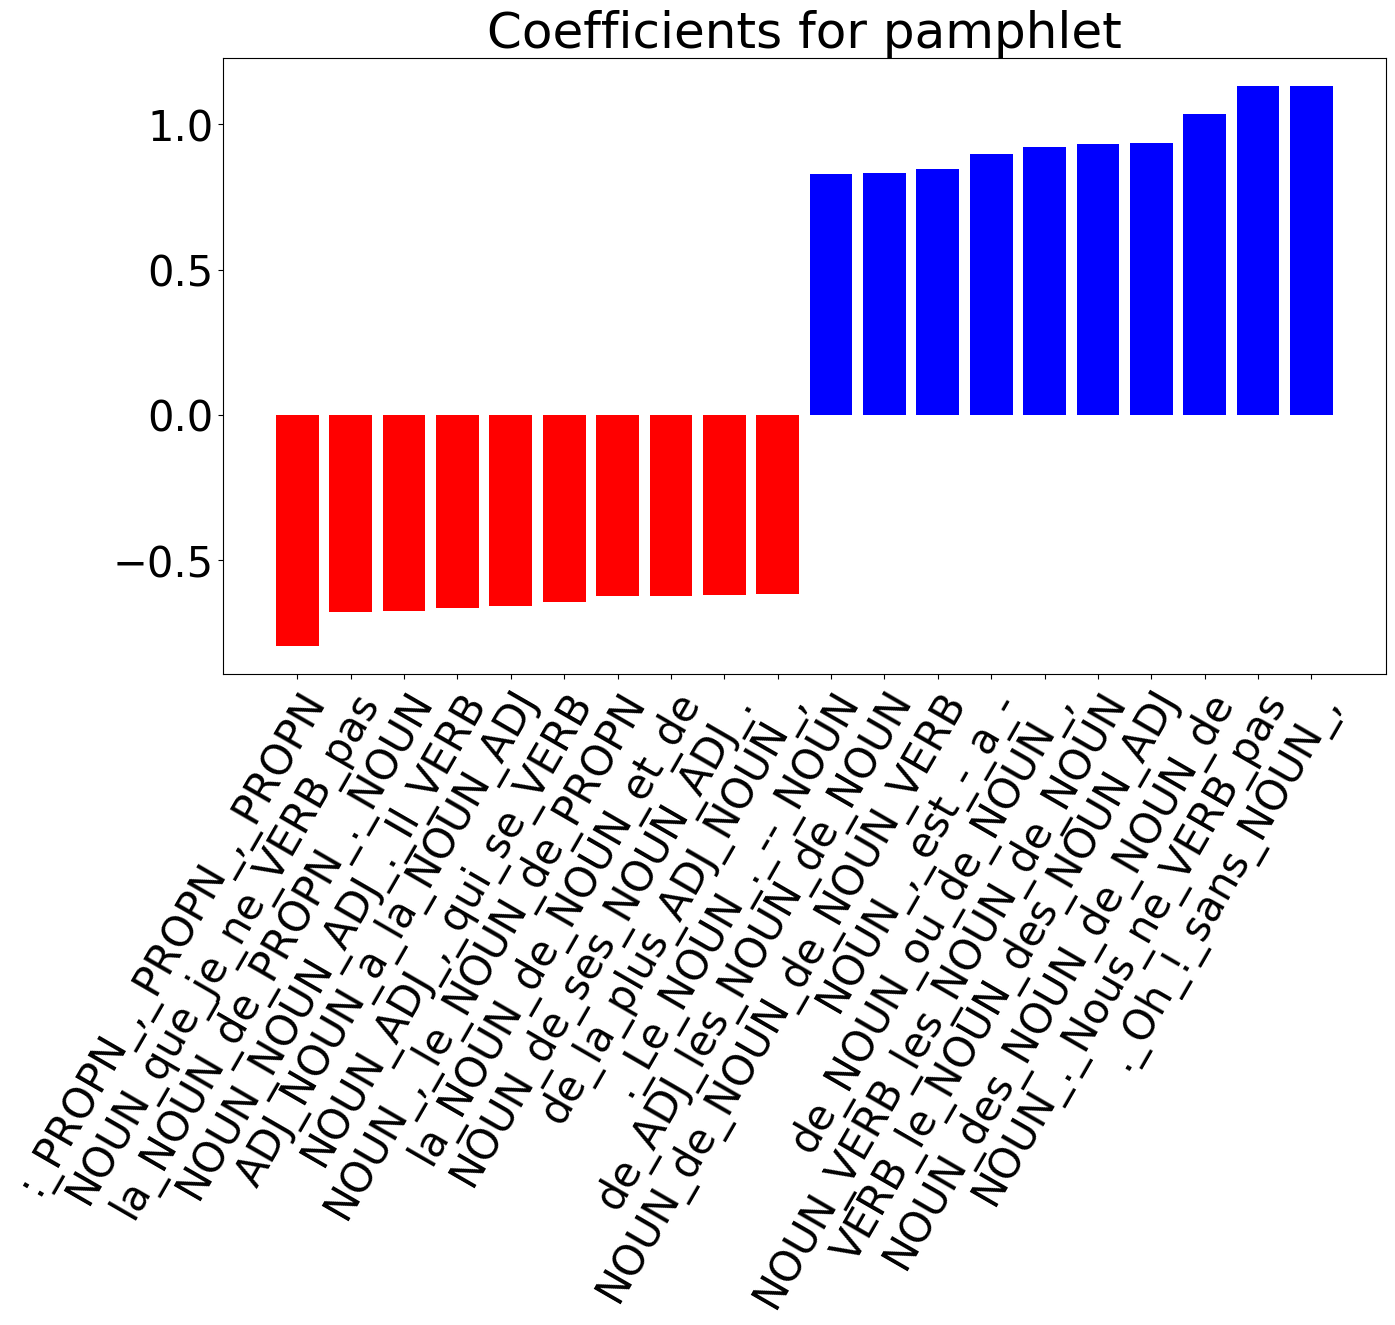
\includegraphics[width=0.70\textwidth]{img/coefs_pamphlet_corpus2restreint.png}
\caption{\textit{Diagramme à barres des coefficients de la classe pamphlet du corpus 2 restreint de motifs}}
\label{'fig:coefs_pamphlet_corpus2restreint'}
\end{figure}

\begin{figure}[H]
\centering %
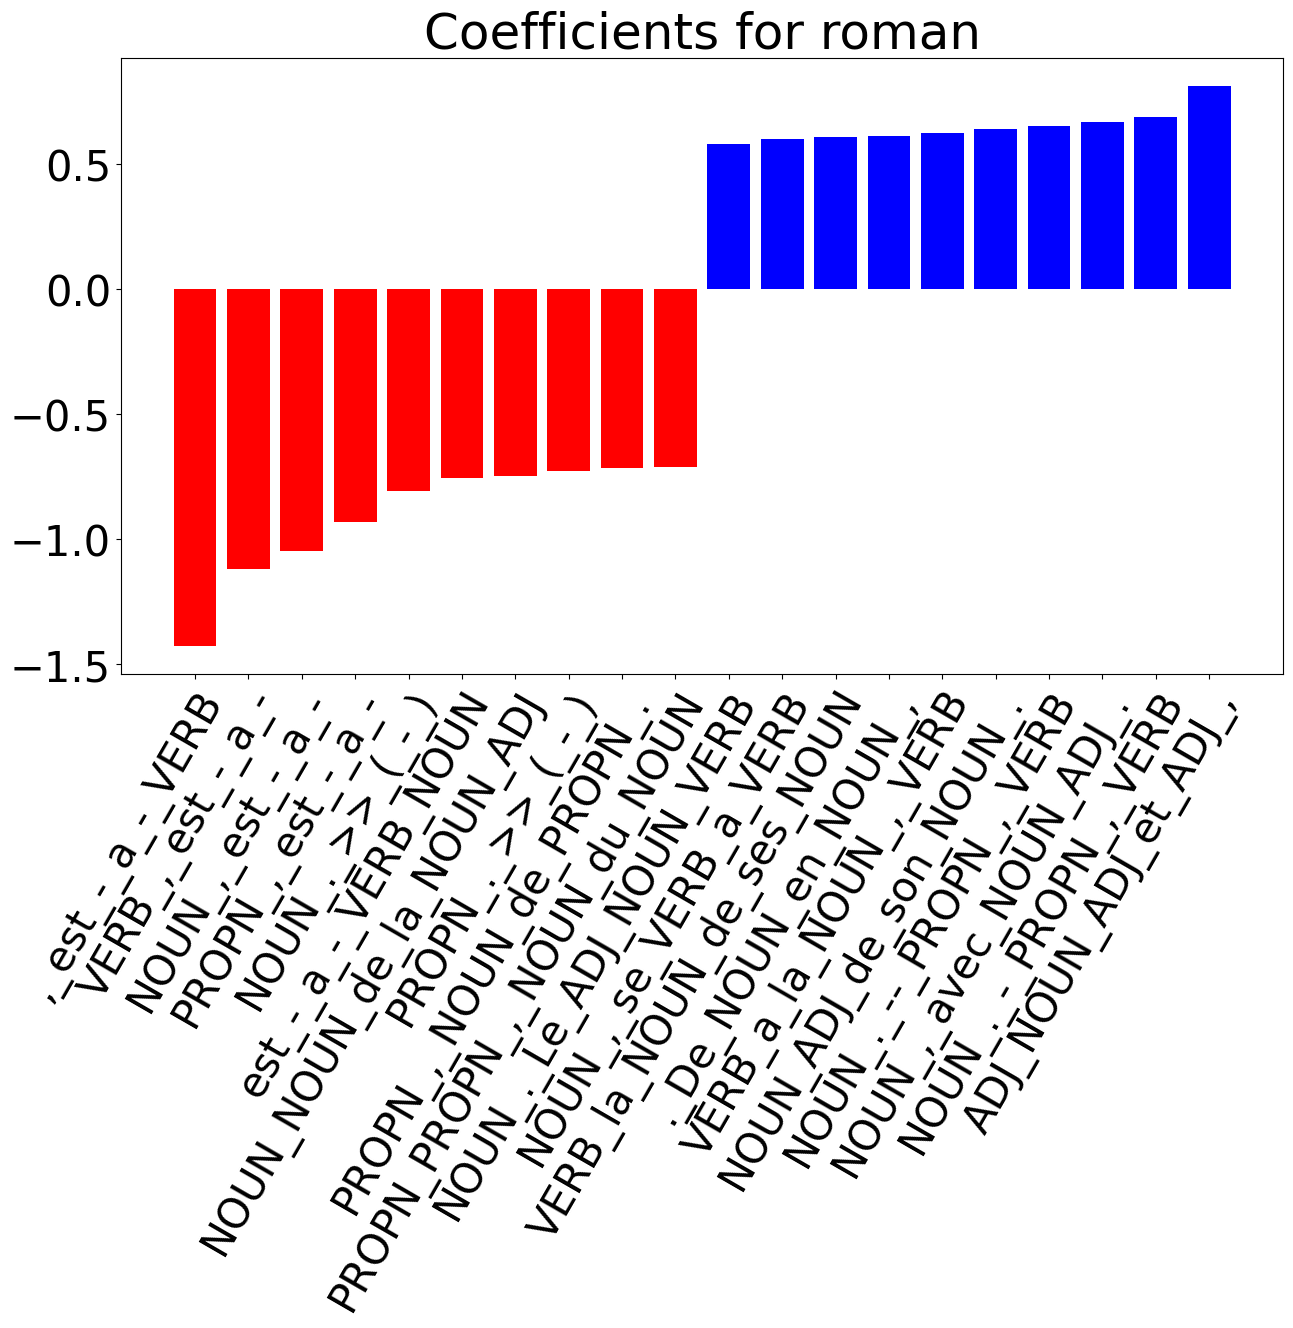
\includegraphics[width=0.70\textwidth]{img/coefs_roman_corpus2restreint.png}
\caption{\textit{Diagramme à barres des coefficients de la classe roman du corpus 2 restreint de motifs}}
\label{'fig:coefs_roman_corpus2restreint'}
\end{figure}

\begin{figure}[H]
\centering %
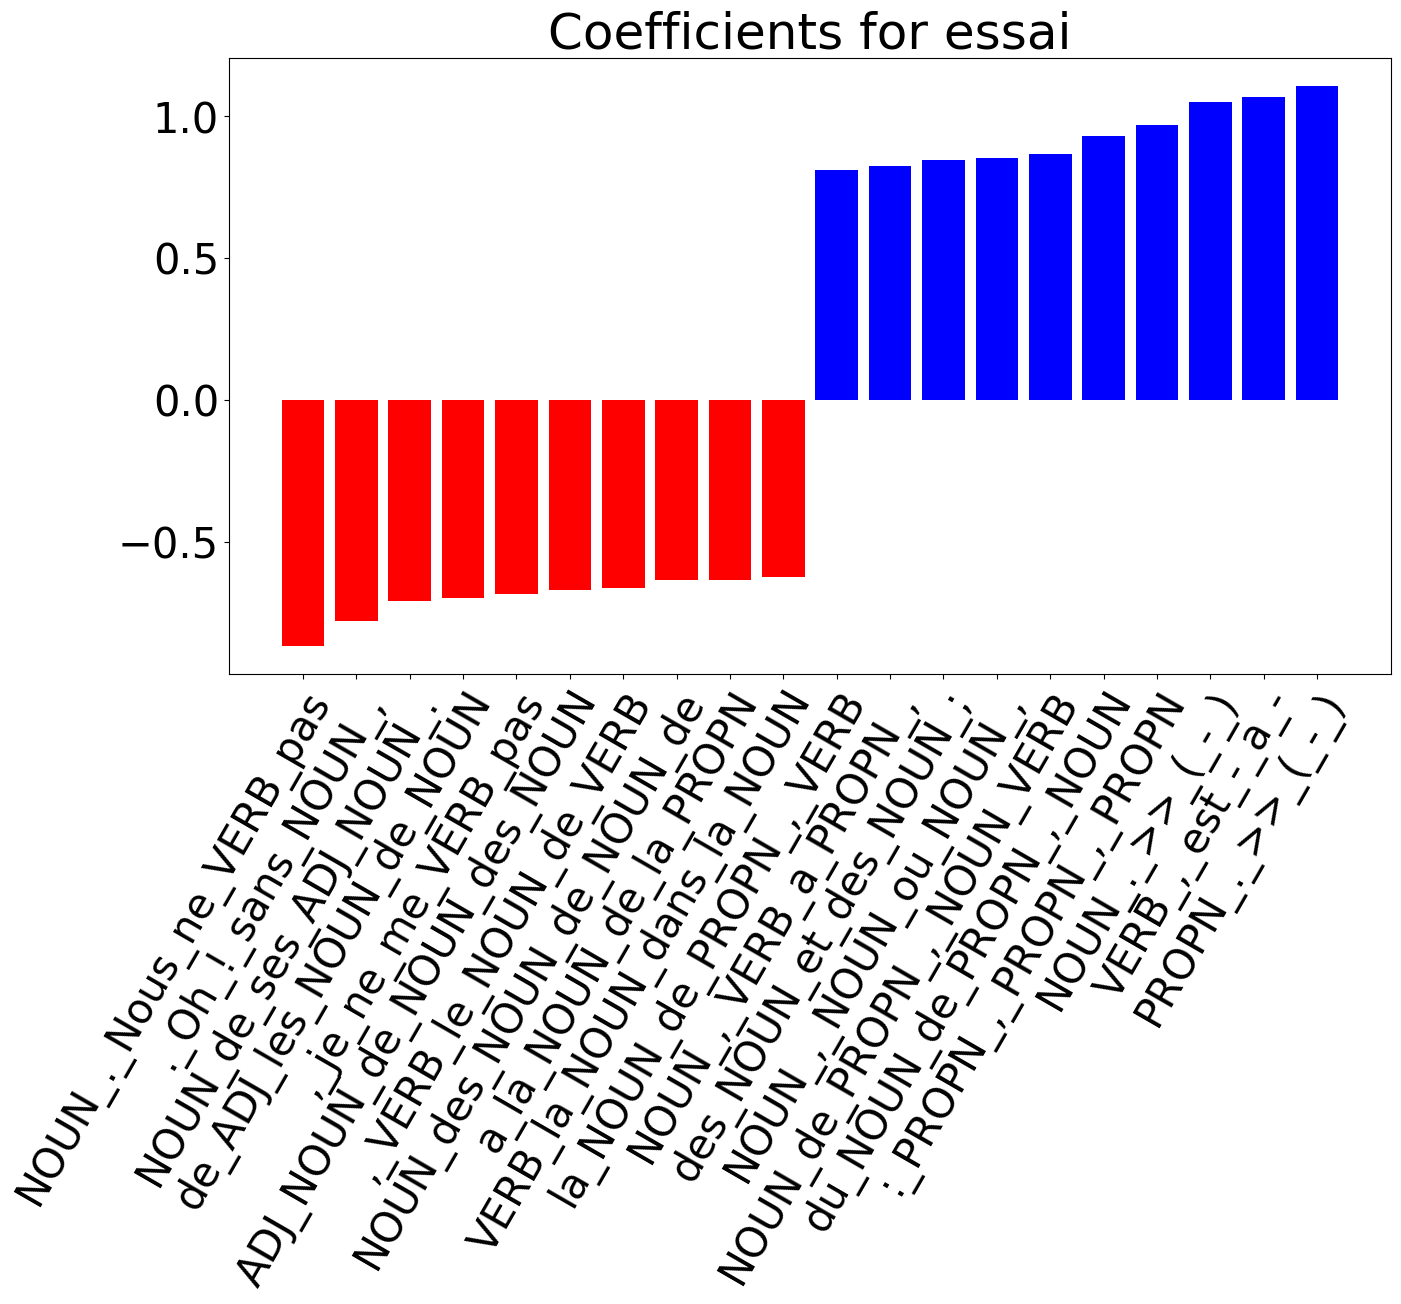
\includegraphics[width=0.70\textwidth]{img/coefs_essai_corpus2restreint.png}
\caption{\textit{Diagramme à barres des coefficients de la classe essai du corpus 2 restreint de motifs}}
\label{'fig:coefs_essai_corpus2restreint'}
\end{figure}

Nous présentons avec la \textit{table \ref{'tab:NOUNoudeNOUN'}} un exemple de ce qu'un des motifs peux dévoiler lorsque l'on recherche les valeurs propres non grammaticalisées dans les textes. La forme déterminant/nom/ou/déterminant/nom dévoile une structure binaire a deux valeur. Soit par opposition comme \enquote{\textit{de vie ou de mort}}, \enquote{\textit{de gré ou de force}} et \enquote{\textit{de paysans ou de bourgeois}}, soit par amplification ou requalification tel \enquote{\textit{de duché ou de comté}}, \enquote{\textit{de médisances ou de calomnies}} et \enquote{\textit{de traîtres ou de lâches}}. Il est intéréssant de voir qu'à travers un même syntagme, différents emplois soit possible.

\newgeometry{left=0.5cm, right=0.5cm}
\begin{longtable}{| p{12.5cm}| c | c| }
    \centering
        \textbf{Match Texte} & \textbf{Nom du Fichier} \\
        \hline
        de système ou de parti & pamphlet\_Bernanos\_La liberté, pour quoi faire \\
        \hline
        de hausse ou de baisse & pamphlet\_Chirac\_Les rois de la République I \\
        \hline
        de tour ou de collection & pamphlet\_Barrès\_Une visite à l’armée anglaise \\
        \hline
        de banditisme ou de forfaiture & pamphlet\_Bloy\_Je m’accuse \\
        \hline
        de vie ou de mort & pamphlet\_Darien\_La Belle France \\
        \hline
        de traîtres ou de lâches & pamphlet\_Bernanos\_Les Grands Cimetières sous la lune \\
        \hline
        de fête ou de dimanche & pamphlet\_Taxil\_Les Pornographes sacrés \\
        \hline
        de régénération ou de destruction & pamphlet\_Taxil\_Les frères Trois-Points \\
        \hline
        de monuments ou de ruines & pamphlet\_Céline\_Mea Culpa \\
        \hline
        de crainte ou de scrupules & pamphlet\_Barrès\_Scènes Et Doctrines Du Nationalisme \\
        \hline
        de variole ou de choléra & pamphlet\_Céline\_Les beaux draps \\
        \hline
        de chefs ou de camarades & pamphlet\_Barrès\_Les Diverses familles spirituelles de la France \\
        \hline
        de croix ou de fleur & pamphlet\_Taxil\_La lanterne d’un suspendu \\
        \hline
        de rouge ou de noir & pamphlet\_Bernanos\_Le crépuscule des vieux \\
        \hline
        de coalitions ou de collusions & pamphlet\_Darien\_Les Vrais Sous-Offs \\
        \hline
        de grains ou de fruits & pamphlet\_Tailhade\_La Noire Idole \\
        \hline
        de perles ou de diamants & pamphlet\_Chirac\_L'agiotage sous la troisième république I \\
        \hline
        de lait ou de pain & pamphlet\_Céline\_Bagatelles pour un massacre \\
        \hline
        de races ou de religions & pamphlet\_Taxil\_À bas la calotte \\
        \hline
        de pions ou de dévotes & pamphlet\_Bernanos\_Où allons-nous \\
        \hline
        de gré ou de force & pamphlet\_Chirac\_L'agiotage sous la troisième république II \\
        \hline
        de chômage ou de bas & pamphlet\_Bernanos\_La France contre les robots \\
        \hline
        de couleur ou de passion & pamphlet\_Tailhade\_À Travers les Grouins \\
        \hline
        de concorde ou de discorde & pamphlet\_Daudet\_La France en alarme \\
        \hline
        de paysans ou de bourgeois & pamphlet\_Vallès\_L'argent \\
        \hline
        de rue ou de café & pamphlet\_Bernanos\_La révolte de l'esprit \\
        \hline
        de comédies ou de drames & pamphlet\_Bloy\_Propos d’un entrepreneur de démolitions \\
        \hline
        de cirage ou de savonnette & pamphlet\_Bernanos\_Le Chemin de la Croix-des-âmes \\
        \hline
        de créancier ou de débiteur & pamphlet\_Chirac\_Les Mystères du crédit \\
        \hline
        de goujatisme ou de piedplatisme & pamphlet\_Bloy\_Devant les cochons \\
        \hline
        de rentes ou de titres & pamphlet\_Tailhade\_Au pays du Mufle \\
        \hline
        de duché ou de comté & pamphlet\_Chirac\_Les rois de la République II \\
        \hline
        de stoïques ou de saints & pamphlet\_Bernanos\_Les enfants humiliés  \\
        \hline
        de chantiers ou de terrains & pamphlet\_Bloy\_Exégèse des lieux communs \\
        \hline
        de guerre ou de salut & pamphlet\_Bernanos\_Francais si vous saviez \\
        \hline
        de droite ou de gauche & pamphlet\_Céline\_L'École des cadavres \\
        \hline
        de cour ou de cuisine & pamphlet\_Chirac\_Erreur commise au préjudice du Trésor français \\
        \hline
        de médisances ou de calomnies & pamphlet\_Taxil\_Mémoires d’une ex-palladiste parfaite, initiée, indépendante \\
        \hline
        de ministre ou de rapporteur & pamphlet\_Chirac\_Les pots de vin parlementaires \\
        \hline
    \caption{Liste de NOUN ou de NOUN pamphlet}
    \label{'tab:NOUNoudeNOUN'}
\end{longtable}


\section{Conclusion}

Nous aurions aimé aller beaucoup plus loin sur cette analyse des motifs, notamment en associant automatiquement les termes lexicalisés à des thèmes en vectorisant les noms, adjectifs et verbes et les plaçant sur des échelles de valeurs comme noble/ignoble, insultant/laudateur et autre. Nous aurions utilisé la librairie Gensim en python pour cela. Cela aurait permis de maximiser la recherche de motifs en associant des valeurs thématiques à des motifs grammaticaux, apportant une dimension de différentes connotations aux motifs.